\chapter{Projekt}
\section{Architektura}
Architektura rozwiązania. Aplikacja stworzona będzie w architekturze klient-serwer. Interfejs użytkownika zrealizowany będzie w technolgii aplikacji internetowych, tak by dostęp do repozytorium nie wymagał instalacji i był dostępny na wszystie platformy. Dodatkowo stworzona zostanie usługa internetowa ( ang. web service ), tak by umożliwić zintegorowanie aplikacji z zewnętrznymi aplikacjami dzięki czemu możliwa będzie automatyzacja kluczowych procesów. Perzystencja danych dokonywana będzie w relacyjnej bazie danych poprzez moduł odwzorowujący obiektową architekturę systemu informatycznego na bazę danych.

Aplikacja zostanie napisana w języku JAVA. Język ten jest obecnie najczęśniej spotykanym językiem w zagadnieniach korporacyjnych. Posiada rozwinięte wsparcie społeczności i rozbudowane funkcjonalności wbudowane, jak i rozwijane przez zewnętrznych kontrybutorów. 
\begin{figure}[h]
\centerline{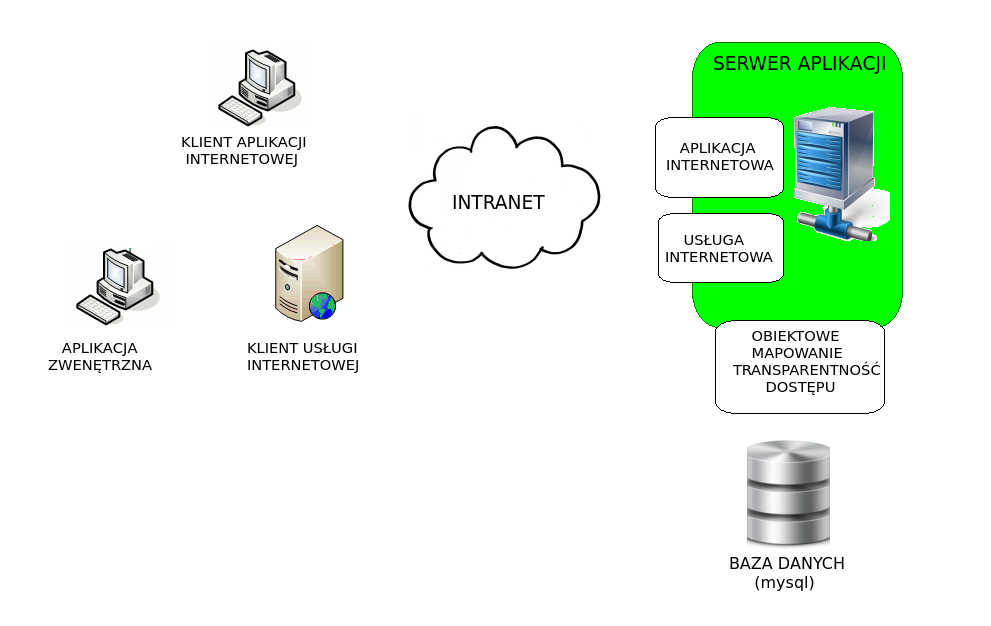
\includegraphics[scale=0.5]{img/architektura.png}}
\caption{Architektura systemu}
\label{fig:architektura}
\end{figure}


%<< Diagram fizyczny >>

%<< Diagram komponentów >>

%Komponent zarządzanie użytkownikami

%Komponent Definicji 

%Komponent wykonania testów

%Komponent danych dodatkwych
\section{Warstwy}
\subsection{Warstwa aplikacji internetowej}
Dostęp poprzez aplikację internetową jest podstawowym źródłem interakcji użytkowika w projektowanej aplikacji. Celem rozdzielenia poszczególnych odpowiedzialności modułów oprogramowania, użyty zostanie zworzec Model-Widok-Kontroler. Zakłada on wydzielenie trzech wartst:
\begin{enumerate}
  \item Model - odpowiedzialny za pobranie i enkapsulacje danych
  \item Widok - odpowiedzialny za wyświetlenie sformatowanej treści. Język stosowany w widoku powinien pozwalać na swobodne osadzanie treści języka końcowego ( w tym przypadku HTML ), powinien on być dostosowany do edycji przez osoby nie posiadające wiedzy na temat języku programowania.
  \item Kontroller - odpowiedzialny za skoordynowanie pobrania danych, przetworzenia ich za pomocą serwisów i przesłanie danych do widoku
\end{enumerate}

Język JAVA oferuje kilka ustandaryzowanych technologii które pozwalają tworzyć aplikacje internetowe z wykorzystaniem wzorca Model-Widok-Kontroler. Zaprezentowana aplikacja stworzona zostanie w oparciu o technologię Java Server Faces i jej implementacje PrimeFaces.

Java Server Faces jest jednym ze standardów tworzenia aplikacji internetowych w języku JAVA\cite{jsfRef}. Główne założenia standardu to:
\begin{enumerate}
  \item Łatwość tworzenia części klienckiej ( widoku ) w oparciu o strukturę komponentową. Udostępnione są standardowe komponenty ( takie jak na przykład formularz, pole tekstowe ).
  \item Możliwość zagnieżdżania struktury dokumentu, pozwalająca na minimalizację redundancji po stronie szablonu strony internetowej 
  \item Ustandaryzowany dostęp z widoku do danych po stronie serweru
  \item Zapewnienie trwałości stanu danych pomiędzy żądaniami w obrębie sesji klienta
  \item Część serwerowa oparta jest na ziarnach ( JavaBeans ), posiada wsparcie dla walidacji zarówno po stronie klienckiej jak i serwerowej
\end{enumerate}

W technologii Java Server Faces rola Kontrolera rozdzielona jest na pliki szablonu strony i ziarna zarządzające po stronie serweru. W plikach szablonu osadzone są instrukcję które wprost pobierają danę z kontrolera i wykonują na nim akcje.

Standard Java Server Faces posiada wiele implementacji. W tworzonej aplikacji użyta została implementacja PrimeFaces\cite{primeFaces}. PrimeFaces jest rozwijany jako otwarty projekt. Implementacja ta rozszerza standard o własne komponenty, uproszcza również sposób komunikacji klient serwer poprzez AJAX ( asynchroniczna komunikacja poprzez język JavaScript)

\subsection{Warstwa usługi internetowej}

Przedsiębiorstwa informatyzują wiele kluczowych procesów biznesowych. Zdarza się iż do rozwiązania konkretnego przypadku stosowane jest kilka różnych systemów, pochodzących od jednego wydawcy lub wydawaców ze sobą niezwiąnych. Fakt istnienia różnych systemów powoduje konieczność zintegrowania ich wspólnie tak by systemy mogły w sposób zautomatyzowany wymieniać między sobą dane, zdarzenia, komunikaty.

Różnorodność na rynku informatycznym powoduje iż programy pracujące w tej samej domenie, używane wspólnie do rozwiązania konkretnej potrzeby biznesowej, tworzone są w różnych technologiach, w odmiennych językach programowania. Potrzeba komunikacji pomiędzy programami, które różnią się implementacją i technologiami rozwiązywana jest poprzez zastosowanie standardów które mogą być stosowane interdyscyplinarnie.

Jedym ze standardów komunikacji między aplikacjami jest komunikacja poprzez usługę internetową, dla której istnieje wiele technologii. W niniejszej pracy użyta zostanie technologia REST. REST zakłada iż deklaracja działania które klient zamierza osiągnąć po stronie serwera określona jest w dwóch miejscach:
\begin{enumerate}
  \item URI czyli adres interntetowy określa do którego zasobu odwołuje się klient
  \item  typ metody HTTP ( zgodnie z HTTP/1.1) określa jakie działanie ma być podjęte na zasobie ( wyświetlenie, dodanie, modyfikacja, usunięcie)
\end{enumerate}

Zgodnie ze specyfikacją HTTP/1.1 możemy wyróżnić następujące metody i oczekiwany rezultat po stronie serwerowej:

\begin{table}	
	\centering
\begin{tabular}{|c|c|}
\textbf{metoda} & \textbf{mapowanie na akcje} \\ \hline
GET & Wyświetlenie, pobranie zasobu \\ \hline
PUT & Stworzenie zasobu \\ \hline
POST & Modyikacja zasobu \\ \hline
DELETE & Usunięcie zasobu \\ \hline
OPTIONS, TRACE, HEAD & nie używane \\ \hline
\end{tabular}
\caption{Metody HTTP/1.1 \cite{http}}
\end{table}

Poprzez usługę internetową możliwe będzie wykonanie następujących akcji:
\begin{enumerate}
  \item dodanie wymagania
  \item pobrania listy przypadków testowych do wykonania dla użytkownika
  \item aktualizacji wykonania przypadku testowego
\end{enumerate}
Pierwszy punkt pozwala na integracje z aplikacją przechowującą wymagania. Punkt drugi i trzecie pozwala na integracje z zewnętrznymi aplikacjami do wykonywania testów. W szczególnym przypadku poprzez stworzenie fikcyjnego użytkownika np. automatyzacja, można zintegrować repozytorium z modułem wykonującym testy automatycznie.


\subsection{Moduły aplikacji}
Funkcjonalności realizowane przez aplikację możemy podzielić na logicznę moduły.
\begin{figure}[h]
\centerline{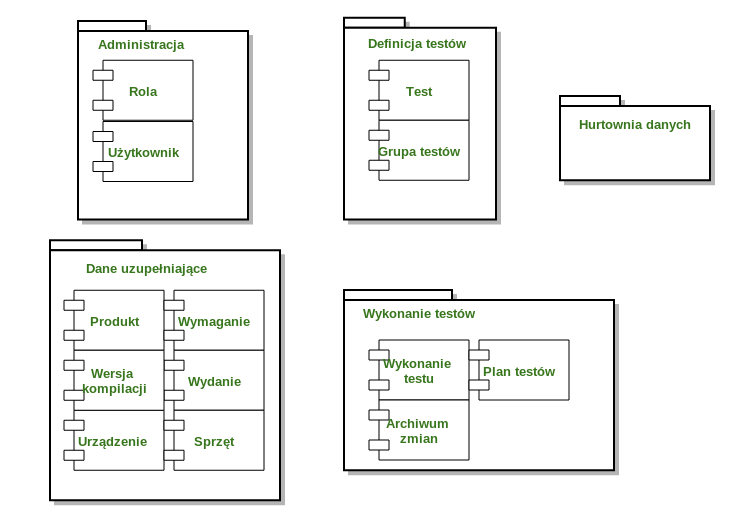
\includegraphics[scale=0.5]{img/komponenty.png}}
\caption{Mouły systemu}
\label{fig:moduly}
\end{figure}

\subsubsection{Moduł administracji}

Moduł ten skupia wszelkie funkcjonalności związane z zarządzaniem użytkownikami w systemie. Odpowida za tworzenie i edycję użytkowników. Każdy użytkownik posiada takie dane jak login, adres e-mailowy, hasło jak również przypisaną rolę.

Możemy wyróżnić kilka ról użytkowników. Rola określa jakie uprawnienia otrzymuje zalogowany użytkownik i określa widok ekranu początkowego. Każda z ról posiada charakterystyczne cechy które pokrywają role użytkowników w procesie testowania oprogramowania: menedżer testów, lider testów, inżynier testów, specjalista środowiska do testów, specjalista konfiguracji testowej \cite{peopleWare}. Poniżej zaprezentowany zostanie opis poszczególnych ról.
\begin{enumerate}
  \item Administrator --  zarządza użytkowikami w systemie. Administrator tworzy użytkowników i nadaje im uprawnienia.
  \item Koordynator testów -- tworzy przypadki testowe, grupy testów i plany testów. Rola ta odpowiedzialna jest za treści merytoryczne repozytorium. Użytkownik odpowiada za utrzymanie testów, aktualizację ich, pokrycie funkcjonalności. 
  \item Obsługa techniczna -- rola ta odpowiedzialna jest za zapewnienie odpowiedniego środowiska dla testerów, konserwacje i naprawę fizycznych defektów. Użytkownik ten przypisany jest do konkretnych wykonań scenariuszy, instaluje początkowe środowisko, wymagane wersje oprogramowania, naprawia usterki sprzętowe.
  \item Lider testów -- wspiera zespół w wykonynwaniu planu testów testowego. Służy swoją wiedzą i doświadczeniem przy podziale prac i podczas pojawiających się problemów. Posiada władzę decyzyjną przy zakwalifikowaniu testu jako nie udanego. Lider przypisuje testerów do testów.
  \item Tester --  wykonuje przypisane do niego przypadki testowe. Odznacza stan testów i zgłasza napotkane problemy.
  \item Pośrednik ( ang. liaison ) --  Odpowiedzialny jest za komunikacje zespołu testów z zespołem programistycznym. Posiaga wgląd do aktulnie wykonywanyh testów i konfiguracji. Jego zadaniem jest rozwiązywanie problemów związanych z jego macierzystym produktem. Pomaga zakwalifikować problem powstały podczas testów, szczególnie na początku testów produktu, zespół testerki może nie posiadać wystarczającej wiedzy i błędnie kwalifikować obserwowane rezultaty jako błąd produktu. Pośrednik proponuje również tymczasowe rozwiązania które pozwalają obejść problemy wynikające z błędów w oprogramowaniu, które naprawione będą dopiero podczas przyszłych wersji oprogramowania, tak by proces testowania mógł przebiegać nieprzerwanie.
\end{enumerate}
  
\subsubsection{Moduł definicji}

Moduł ten jest odpowiedzialny za definicję podstawowych jednostek systemu czyli: testów, grup testów i planów testów. 

Podstawową jednostą aplikacji jest przypadek testowy. Składowe:
\begin{enumerate}
  \item tytuł
  \item identyfikator
  \item abstrakt czyli opis testu, jego kluczowe założenia pozwalające wdrożyć się testerowi w temat
  \item grupy urządzeń. Do jednej grupy urządzeń może być przypisane jedno lub więcej urządzeń ( w przypadku gdy dana funkcjonalność adresowana jest na więcej niż jedno urządzenie). Podczas wykonania testu należy jednak określić którego urządzenia z grupy należy użyć
  \item stan wejściowy konfiguracji. Definiowane jest tutaj sprzęt i jego stan który jest wymagana do wykonania testu. Dla każdego ze stanów można zdefiniować warunek określający dla jakich konfiguracji grup urządzeń stan ma zajść
  \item scenariusz, to jest lista kroków do wykonania wraz z oczekiwanymi rezultatami
  \item wymagania które są weryfikowane przez wykonanie testu
  \item estymowany czas potrzebny do wykonania przypadku testowego
  \item stan początkowy poszczególnych produktów który musi być spełniony. Dla każdego ze zdefiniowanych stanów możliwe jest przypisanie warunku który określa dla jakiej konfiguracji grup urządzeń stan ma zajść
\end{enumerate}

Przypadki testowe wchodzą w skład grup testów. Hierarchia ta ma drzewiastą strukturę co oznacza iż grupy mogą być zagnieżdżane. Grupy powinny agregować testy które posiadają podobną charakterystykę. Na przykład testują te same funkcjonalności, wymagają podobnej konfiguracji, urządzeń, dokumentacji. Testy funkcjonalne i niefunkcjonalne nie powinny znajdować się w tym samym przypadku testowym. Składowe:
\begin{enumerate}
  \item  tytuł
  \item identyfikator
  \item identyfikator rodzica
  \item opis
\end{enumerate}

Podczas trwania procesu wytwarzania oprogramowania należy wybrać z puli istniejących testów, te które będą wykonywane przez zespół. Dokument definiujący co należy przetestować i przy pomocy których przypadków użycia nazywamy przypadkiem testowym. Oto jego składowe w systemie:

\begin{enumerate}
  \item tytuł
  \item opis, dlaczego plan jest wykonywany, jego cel i oczekiwane rezultaty
  \item lista wymagań które pokrywa plan 
  \item lista urządzeń które będą dostępne podczas testów
  \item referencja do wersji produktu dla której wykonywane będą testy 
\end{enumerate}

\subsubsection{Moduł danych uzupełniających}

Definicja testów przez swoją złożoność i potrzebę pełnej specyfikacji wymaga pewnych danych dodatkowych które muszą zostać zdefiniowane w aplikacji.

Repozytorium przezonaczone jest dla systemów wielo wydaniowych. Dodatkowo wspierany jest inkrementacyjny model wytwarzania oprogramowia. W celu spełnienia przedstawionych funkcjonalności w systemie istnieją takie elementy jak "wydanie produktu" i "wersja produktu" która wchodzi w skład wydania. Poprzez wersje produktu rozumiany jest konkretny skompilowany stan kompontów systemu, jednoznacznie identyfikowany który stanowić będzie linie bazową sytemu wdrożonego w środowisku testowym. 

W ramach wydań produktów definiowane są wymagania. Wymaganie powinno być jasno zdefiniowane tak by możliwe było zweryfikowanie spełnienia wymagania przez oprogramowanie. Na podstawie wymagań tworzone są przypadki testowe.

Drugą charakterystyką aplikacji jest wsparcie dla systemów dedykowanych na wiele urządzeń. Aplikacje umożliwia więc przechowywanie informacji o urządzeniach. Definicja urządzenia powinna zawierać dane podstawowe takie jak nazwa, dostawca, zdjęcie jak i referencję do kompletnej dokumentacji na temat urządznia. Dostę do dokumentacji jest kluczowy podczas testów, szczególnie dla młodego stażem personelu.

W module definicji testów, podczas tworzenie przypadku testowego tworzone są grupy urządzeń. W skład grupy może wejść jedno lub więcej urządzeń, przy czym podczas wykonania przypadku testowego należy wybrać tylko jedno urządzenie dla każdej z grup. Konfiguracja wybranych urządzeń determinuje i modyfikuje końcową treść przypadku testowego. Od tego które urządzenia zostały wybrane mogą zależeć poszczególne kroki, stany początkowe produktów i wymagany sprzęt. Aplikacja repozytorium udostępnia sposób definiowania warunków dla wcześniej wspomnianych elementów. Warunek określa iż dany element jest ważny ( wchodzi w skład definicji przypadku testowego) wtedy i tylko wtedy gdy dla określonej grupy urządzeń wybrane zostało określone urządzenie.



\subsubsection{Moduł wykonania }

Moduł ten przechowuje elementy odpowiadające wykonanym i oczekującym do wykonania przypadkom testowym. W celu rozpoczęcia testów należy utworzyć plan testów, określić zakres, wymagania które będą weryfikowane jak i dostępny sprzęd i urządzenia.

Po definijci planu testowego należy dobrać testy które zostaną wykonane, wybóru należy dokonać biorąc po uwagę potrzebe spełnienia planu przy określonych zasobach ludzkich.

Definicja testów jak już zostało wcześniej wspomniane pozwala na warunkowe określnenie pewnych elementów w zależności od końcowej konfiguracji na którą dedykowany jest przypadek testowy.

	\begin{codebox}
	\li \For{$stanProduktu$ \kw{in} $stanyProduktu$}
	\li \Do   
	\For{$warunek$ \kw{in} $warunkiDlaGrupUrzadzen$}
	\li \Do
	     \If $wybraneUrzadzenie  !=  preferowaneUrzadzenieDlaStanu$
	\li     \Then
	          $\proc{PRZERWIJ}$
	          \Else
	          $\proc{dodaj-stan-do-testu}(stanProduktu)$
	        \End
	        
	\li  \End
	 
	\li
	  \End
	\end{codebox}

\subsubsection{Moduł hurtowni danych  }


\section{Składowe aplikacji}

\chapter{Implementacja}
Interfejs użytkownika stworzony został w technologi aplikacji internetowych przy użyciu technologii Java Server Faces która realizuje wzorzec projektowy  Model-Widok-Kontroler. Warstwa serwerowa działa na serwerze aplikacji Glassfish. Silnik bazodanowy to Mysql, silnik ten może być zmieniony podczas wdrożenia aplikacji poprzez zastosowanie tranparentności dostępu do danych. Moduł odwzorowujący obiektową architekturę systemu informatycznego na bazę danych udostępnia wiele implementacji baz danych przy czym interfejs jest wspólny.

\section{Workflow}
\begin{enumerate}
  \item Tworzony jest nowy projekt
  \item Tworzone są wymagania
  \item Na podstawie wymagań tworzone są grupy testów i przypadki testowe. Scenariusze przypadków testowych tworzone są przy współpracy z zespołem programistycznym.
  \item Tworzony jest nowy plan testów który testować będzie nowe wydanie produktu. Tworzony jest harmonogram uwzlględniający poszczególne inkrementy produktu i testowane funkcjonalności.
  \item Do planu testów dodawane są testy. Podczas dodawania testów należy wziąć pod uwagę pokrycie nowych funkcjonalności i równomierne rozplanowanie testów dla różnych urządzeń.

\end{enumerate}
